%%%%%%%%%%%%%%%%%%%%%%%%%%%%%%%%%%%%%%%%%%%%%%%%%%%%%%%%%%
\documentclass[xcolor=pdftex,dvipsnames,table,10pt]{beamer}
%handout, if no \pause

\usepackage{tabularx}
\usepackage[]{algorithm2e}
\usepackage{listings}
\usepackage{lstautogobble}

%\documentclass[handout,xcolor=pdftex,dvipsnames,table]{beamer} % USE THIS WITH pdfpages STUFF
%\usepackage{pgfpages}
%\pgfpagesuselayout{resize to}[a4paper, landscape]

\definecolor{headerColour}{RGB}{180, 230, 245}
\definecolor{headerTitleColour}{RGB}{0, 60, 80}
\definecolor{sectionShadedColour}{RGB}{50, 110, 130}
\definecolor{subsectionHighlightColour}{RGB}{50, 50, 50}
\definecolor{subsectionShadedColour}{RGB}{100, 100, 100}

\setbeamercolor{subsection in sidebar}{fg=subsectionHighlightColour}
\setbeamercolor{subsection in sidebar shaded}{fg=subsectionShadedColour}
\setbeamercolor{structure}{fg=headerTitleColour, bg=headerColour}
\setbeamercolor{title}{fg=headerTitleColour, bg=white}
\setbeamercolor{section in sidebar shaded}{fg=sectionShadedColour}

\usetheme{Goettingen}
\makeatletter\setbeamertemplate{sidebar canvas \beamer@sidebarside}[vertical shading][top=headerColour,bottom=white]\makeatother

%% to suppress subsections in sidebar:
%\setbeamertemplate{subsection in sidebar shaded}
%{\vspace*{-\baselineskip}}
%\setbeamertemplate{subsubsection in sidebar shaded}
%{\vspace*{-\baselineskip}}

\usepackage{amsmath, amssymb}
\usepackage{fancyvrb}


% Font modification
\usefonttheme{professionalfonts}
\usepackage{cmbright}
\usepackage{eulervm}
\newfont{\Ss}{cmcsc12 scaled 1600}

% no navigation symbols at the bottom of frames
\beamertemplatenavigationsymbolsempty
\setbeamertemplate{footline}[frame number] 

\usepackage{subcaption}

\usepackage{multirow} % allows entries across multipe rows in tables
\usepackage{booktabs} % makes fancier rulers in tables
%\usepackage{setspace} % spacing between lines

%%%%%%%%%%%%%%%%%%
%% Bibliography related stuff:
% control space between lines
  \let\oldthebibliography=\thebibliography
  \let\endoldthebibliography=\endthebibliography
  \renewenvironment{thebibliography}[1]{
    \begin{oldthebibliography}{#1}
      \setlength{\parskip}{-0.5ex}
      \setlength{\itemsep}{-0.5ex}
  }{ \end{oldthebibliography} }
% Force entry to be in one line
\setbeamertemplate{bibliography entry title}{}
\setbeamertemplate{bibliography entry location}{}
\setbeamertemplate{bibliography entry note}{}
% Set bullet point shape:
\setbeamertemplate{bibliography item}{-}
%%%%%%%%%%%%%%


\newenvironment{items}{\begin{list}{$\bullet$}{\itemsep0ex plus 0.2ex
\parsep0ex plus 0.2ex \topsep0ex \parskip0ex}}{\end{list}}
\newcommand{\head}[1]
{\slide{\begin{center}\textbf{#1}\vspace*{-0.5\baselineskip}
{\color{red}\rule{\textwidth}{1mm}}\end{center}}}
\parskip0.3ex

\newcommand{\cT}{{\mathcal T}}


%\defbeamertemplate*{title page}{customized}[1][]
%{
%  \titlepage
%  \usebeamerfont{title}\inserttitle\par
%  \usebeamerfont{subtitle}\usebeamercolor[fg]{subtitle}\insertsubtitle\par
%  \bigskip
%  \usebeamerfont{author}\insertauthor\par
%  \usebeamerfont{institute}\insertinstitute\par
%  \usebeamerfont{date}\insertdate\par
%  \usebeamercolor[fg]{titlegraphic}\inserttitlegraphic
%}



\author[]{Veronika Bo\v{s}kov\'{a} {\scriptsize \& Chi Zhang}}
%\institute{Computational Evolution \\ Department of Biosystems Science and Engineering}
\title[Taming the Beast]{Taming the Beast Workshop \\ \ \\ Priors and starting values} 
\date{June 18, 2018}
\titlegraphic{\hspace*{8cm}
\includegraphics[height=1.5cm]{figures/cEvo_logo_transparent.png}}
%{\small Link to Script\&Slides:  \url{http://www.tb.ethz.ch/education} 
%}

%%%%%%%%%%%%%% Figure caption setup
\usepackage[compatibility=false]{caption}
\captionsetup[figure]{labelsep=space,justification=centering}
\renewcommand{\figurename}{\scriptsize Figure adapted from}

% syntax: \figureCaption{Citation caption}{Second (real) caption}
% second caption can be skipped, first one has to be suppressed if you want to skip it
\newcommand\figureCaption[2]{%
  \captionsetup{aboveskip=0.1cm,belowskip=0cm}
  \caption{\scriptsize #1}
  \caption*{#2}
}

%%%%%%%%%%%%%% Fixme and comment setup§
\definecolor{red}{HTML}{C92D39}
\definecolor{green}{HTML}{498A44}

% syntax: \fixme{What needs to be fixed}
\newcommand{\fixme}[1]{\textcolor{red}{\texttt{{\bf FIX ME:} #1}}}
% Hide all fixmes by switching the line above to this:
%\newcommand{\fixme}[1]{}

% syntax: \comment{Name of commenter}{C omment}
\newcommand{\comment}[2]{\textcolor{green}{{\bf Comment by {#1}}: #2}}
% Hide all comments by switching the line above to this:
%\newcommand{\comment}[2]{}

\definecolor{correct}{HTML}{025B0A}
\definecolor{incorrect}{gray}{0.6}

\newenvironment{questions}{
	\begin{enumerate}[1)]
		\setlength{\itemsep}{1cm}
		\setlength{\parskip}{-0.1cm}
}{\end{enumerate}}

\newenvironment{answers}{
	\begin{enumerate}[a)]
		\setlength{\itemsep}{0cm}
		\setlength{\topsep}{0cm}
		\setlength{\parskip}{0cm}
		\setlength{\parsep}{0cm}
}{\end{enumerate}}

\begin{document}

\begin{frame}
  \titlepage
\end{frame}

\section{Priors and starting values}

%%%%%%%%%%%%%%%%%%%%%%%%%%%%%%%%%%%%%%%%%%%%%%%%%%%%%%%%%%
%%%%%%%%%%%%%%%%%%%%outline%%%%%%%%%%%%%%%%%%%%%%
%%%%%%%%%%%%%%%%%%%%%%%%%%%%%%%%%%%%%%%%%%%%%%%%%%%%%%%%%%
%\begin{frame}\frametitle{Outline of lecture}
%  \begin{itemize}
%   \item EXAMPLE1
%    \begin{itemize}
%    \item[-] EXAMPLE1.1
%    \item[-] EXAMPLE2.1
%    \end{itemize}
%  \end{itemize}
%  \begin{itemize}  
%   \item EXAMPLE2
%    \begin{itemize}
%    \item[-] EXAMPLE2.1
%    \item[-] EXAMPLE2.2
%    \end{itemize}
%  \end{itemize}
%\end{frame}

\subsection{Priors}

\subsubsection{Prior distribution}
\begin{frame}\frametitle{What is a prior?}
	\begin{itemize}
		\item Distribution of a parameter before the data is collected and analysed
		\item as opposed to POSTERIOR distribution which combines the information from the prior and the data
	\end{itemize}
\end{frame}

\begin{frame}\frametitle{What is a prior?}
  \begin{itemize}
  	\item Using Bayes theorem, we can decompose the posterior:
  \end{itemize}
  \begin{figure}[h!]
    \includegraphics<1-1>[height=2.9cm]{figures/posterior.pdf}
    \includegraphics<2-2>[height=2.9cm]{figures/posterior_prior.pdf}
    \includegraphics<3-3>[height=2.9cm]{figures/posterior_priorandtreeprior.pdf}
    \figureCaption{\cite{du2015getting}}{}
  \end{figure}
\end{frame}

\begin{frame}\frametitle{Prior}
	\begin{itemize}
		\item Should not be and is not universal for all the analyses you will ever do in your research 
		%unless you work on a same thing all the time and every experiment you do results into the same conclusions
		\item Should incorporate prior (before looking at the data) knowledge about the parameter/underlying process
		\begin{itemize}
			\item use results of previous independent experiments
			\item use other independent evidence
		\end{itemize}
		\item Should not be too restrictive if prior knowledge/assumptions are weak
		\begin{itemize}
			\item One can use diffuse priors
		\end{itemize}
		\item Prior distribution does not have to, and is not expected to, be exactly the same as the posterior
		\item May not be adjusted after the run, to give higher and higher posterior support
	\end{itemize}
\end{frame}

\begin{frame}\frametitle{Prior}
	\begin{itemize}
		\item Is a choice of 
		\begin{itemize}
			\item model 
			\begin{itemize}
				\item tree-generating models, nucleotide/AA/codon substitution models, ...
			\end{itemize}
		\end{itemize}
		\item[] and of 
		\begin{itemize}
			\item distribution of plausible values for a parameter of interest
			\begin{itemize}
				\item Uniform, Normal, Beta,...
			\end{itemize}
		\end{itemize}
	\end{itemize}
\end{frame}

\begin{frame}\frametitle{Choosing the model}
	\begin{itemize}
		\item To choose the best model
		\begin{itemize}
			\item Use model comparison to choose the one best fitting the data / most adequate for the data
			\item Use rjMCMC (if available) to sample from the posterior distribution including different models. The model where rjMCMC spends the most time (samples the most from), is the best fitting model. 
		\end{itemize}

	\end{itemize}
\end{frame}

\subsubsection{Tree prior}
\begin{frame}\frametitle{Tree prior (tree-generating model)}
	\begin{itemize}
		\item Have to pick one from Coalescent or Birth-death process framework
		\item Have to put priors on parameters of the chosen model
		\begin{itemize}
			\item e.g. growth-rate of the population, R0, extinction rate, ...
		\end{itemize}
	\end{itemize}
\end{frame}

\subsubsection{Substitution model prior}
\begin{frame}\frametitle{Substitution model prior}
	\begin{itemize}
		\item The selection is big: JC69, HKY85, ..., GTR
		\item Use model which has been previously identified to be best for your type of data
		\begin{itemize}
			\item e.g. HKY85			
			\begin{itemize}
				\item Prior for transition/transversion rate ratio ($\kappa$) %\\ (e.g. Gamma)
				\item Prior for base frequencies% (e.g. Dirichlet)
			\end{itemize}	
		\end{itemize}
		\item rjMCMC available in BEAST2 to sample from the posterior distribution including different substitution models (bModelTest)
	\end{itemize}
\end{frame}

\subsubsection{Clock prior}
\begin{frame}\frametitle{Clock prior (molecular clock model)}
	\begin{itemize}
		\item Strict clock: all branches have the same clock rate
		\item Relaxed clock
		\begin{itemize}
			\item Uncorrelated: branches have independent clock rate distributions
			\item Correlated: child branch has clock rate distribution correlated to distribution of the parent branch
		\end{itemize}
	\end{itemize}
\end{frame}

\subsubsection{Parameter prior}
\begin{frame}\frametitle{Parameter prior}
	\begin{itemize}
		\item Can be fixed to a given value \\ (though this is generally not recommended)
		\item Can have upper and lower limits
		\begin {itemize}
			\item If we know that any infected individual recovers after 5-10 days, we can set the distribution of infectious period to be e.g. min 4 days and max 11 days
		\end{itemize}
		\item If specified by a parametric distribution, the parameters of this distribution can also be assigned a prior (hyperprior)
		\item You can visualise the distribution in BEAUti
	\end{itemize}
\end{frame}

\begin{frame}\frametitle{Examples - Normal distribution}
	 \begin{figure}[h!]
   		 \includegraphics<1-1>[height=5cm]{figures/example_normal.pdf}
   	\end{figure}
	\begin{itemize}
		\item Parameters: mean $\mu\in R$, standard deviation $\sigma>0$
		\item Range of values: (-$\infty$,$\infty$)
		\item[]
	\end{itemize}
\end{frame}

\begin{frame}\frametitle{Examples - LogNormal distribution}
	 \begin{figure}[h!]
   		 \includegraphics<1-1>[height=5cm]{figures/example_lognormal.pdf}
   	\end{figure}
	\begin{itemize}
		\item Parameters: mean M $\in R$, standard deviation S $>0$
		\item Range of values: [0,$\infty$)
		\item Long tail, always positive
	\end{itemize}
\end{frame}

\begin{frame}\frametitle{Examples - Beta distribution}
	 \begin{figure}[h!]
   		 \includegraphics<1-1>[height=5cm]{figures/example_beta.pdf}
   	\end{figure}
		\begin{itemize}
		\item Parameters: shape $\alpha>0$, shape $\beta>0$
		\item Range of values: [0,1]
		\item Good for e.g. sampling probability prior
	\end{itemize}
\end{frame}

\begin{frame}\frametitle{Examples - Uniform distribution}
	 \begin{figure}[h!]
   		 \includegraphics<1-1>[height=5cm]{figures/example_uniform.pdf}
   	\end{figure}
		\begin{itemize}
		\item Parameters: lower, upper bound
		\item Range of values: (-$\infty$,$\infty$)
		\item[]
	\end{itemize}
\end{frame}

\begin{frame}\frametitle{Is uniform distribution a non-informative prior?}
	\begin{itemize}
		\item Not really
		\begin{itemize}
			\item Imagine setting a Uniform(0, 100) prior for the transition/transversion rate ratio ($\kappa$). You also know that the most likely values for $\kappa$ are between 0 and 10. But you now put 9/10 of the weight to values $>$ 10.
		\end{itemize}
		\begin{figure}[h!]
    			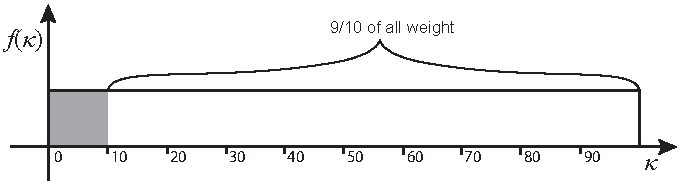
\includegraphics[height=2cm]{figures/9tenths.pdf}
  		\end{figure}
	\end{itemize}
	\begin{itemize}
		\item In fact there is nothing such as an non-informative prior
		\item If little or no information on the parameter is available, use diffuse priors
		\item Try to avoid Uniform(-$\infty$, $\infty$) or Uniform(0, $\infty$)
	\end{itemize}
\end{frame}

\begin{frame}\frametitle{Proper vs improper priors}
	\begin{itemize}
		\item Sometimes the prior distribution is such that the sum or the integral of the prior values does not converge, this is called an IMPROPER prior
		\item Examples
		\begin{itemize}
			\item 1/x
			%\item Beta(0,0)
			\item Uniform($-\infty$,$\infty$)
		\end{itemize}
	\end{itemize}
\end{frame}

\subsubsection{Think twice}
\begin{frame}\frametitle{Are my priors what I set them to be?}
	\begin{itemize}
		\item Not always
		\begin{itemize}
			\item Induced priors may change the picture, i.e. if the parameters interact, the marginal prior distribution for each individual parameter may be different from the originally specified prior
		\end{itemize}
		\item Use sampling from the prior, to see what your 'real' prior is
	\end{itemize}
	\begin{figure}[h!]
		\begin{subfigure}[t]{0.4\textwidth}
		{\label{fig:tbmp:a}
		 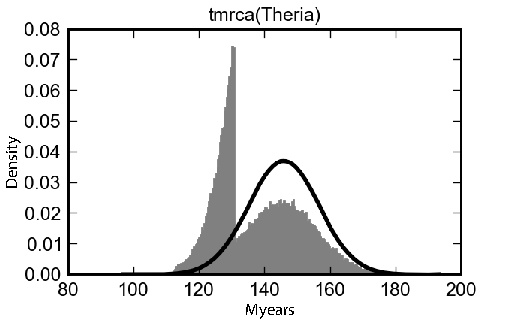
\includegraphics[width=4cm]{figures/tmrca(Theria)-bw.pdf}
		}
		\end{subfigure}
		\begin{subfigure}[t]{0.4\textwidth}
		{\label{fig:tbmp:b}
		 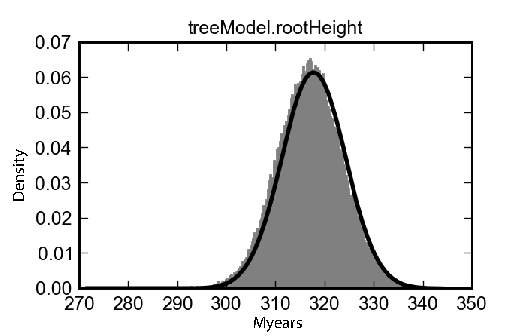
\includegraphics[width=4cm]{figures/treeModel-rootHeight-bw.pdf}
		}
		\end{subfigure}
		\figureCaption{\cite{heled2012calibrated}}{The marginal prior distributions that result from the multiplicative construction (gray) versus calibration densities (black line) specified for the calibrated nodes.}
  	\end{figure}
\end{frame}

\begin{frame}\frametitle{How to choose priors?}
	\begin{itemize}
		\item Use all the prior knowledge you have to choose models and set appropriate parameter priors
		\item Sample from the prior distribution before using your data to check you really have the priors you want
		\item Check your posterior distribution against the prior% - will be elaborated upon on Thursday
	\end{itemize}
\end{frame}

\begin{frame}\frametitle{Word of caution}
	\begin{itemize}
		\item In practice, it is important to evaluate the impact of the prior on the posterior in a Bayesian robustness analysis
		\item Ideally, the posterior should be dominated by your data, such that the choice of the prior has little influence on the result
		\item If this is not the case, the choice of prior is very important, and should be reported
	\end{itemize}
\end{frame}

\subsection{Starting values}

\begin{frame}\frametitle{Starting values}
	\begin{itemize}
		\item Are just starting values
		\item Have to be within the prior distribution, and its upper and lower limits, you chose for the parameter
		\item Use your best guess
		\begin{itemize}
			\item BEAST2 attempts 10 times at most (can be changed) to initialize the run, but if the starting values are unreasonable, the runs may keep failing
		\end{itemize}
		\item Start from different starting values to make sure the chains converge to the same distribution
	\end{itemize}	
\end{frame}


\section{References}
\begin{frame}[t,allowframebreaks]\frametitle{References}
\bibliographystyle{apalike}
\tiny\bibliography{bibliography}
\end{frame}

\end{document}
